%!TEX root = ../thesis.tex
%*******************************************************************************
%*********************************** First Chapter *****************************
%*******************************************************************************

\chapter{Introduction} \label{chapter:introduction}

\ifpdf
    \graphicspath{{Chapter1/Figs/Raster/}{Chapter1/Figs/PDF/}{Chapter1/Figs/}}
\else
    \graphicspath{{Chapter1/Figs/Vector/}{Chapter1/Figs/}}
\fi

TODO:
\begin{itemize}
	\item Last bit of Chapter 5
	\item First introduction in Chapter 1
	\item Explicitly mention which work is my own. Clarify work with Philip
	\item Summary chapters
	\item Add more references
	\item Write dedication
	\item Typo checks
\end{itemize}



New outline:
- GR. Statistical homogeneity and isotropy -> FLRW metric. No static solution.

- Hubble's results. Expanding universe -> Big Bang.

- Discovery of CMB. CMB is a key prediction of Big Bang theory

- Big Bang theory's problem with initial conditions. Inflation. Quantum fluctuations as seeds for inhomogeneities of the universe.

- CMB anisotropy, 1 in $10^5$. Consistent with inflationary predictions.

- Observational evidence for dark energy and dark matter. Emergence of inflationary LCDM.

- LCDM successful. Planck CMB power spectrum -> consistent and measures parameters to percent level. Era of precision cosmology.

- Quick summary of CMB's usefulness! Its existence, anisotropy and spectrum all contributed...  CMB probes initial conditions, growth of the universe and matter distribution (through lensing).

- Next big question - inflation's mechanism? Primordial non-Gaussianity is a robust prediction of many models. Three-point correlation function as a key statistic for differentiation.

- CMB bispectrum. Planck gave a lot of insight. No detection, but oscillatory models are of interest. Main challenge - computational complexity.

- Next generation of CMB experiments upcoming. Polarisation sensitivity improved, higher resolution. Need for development of new, improved pipeline capable of dealing with high resolution data.

- Thesis organisation.

Radio astronomers Arno Penzias and Robert Wilson were calibrating their 50-foot-long horn antenna when they found a mysterious background noise. The measurements were independent of time and location in the sky and persisted after the removal of various potential contaminants. After the theoretical work of Robert Dicke, Jim Peebles, and David Wilkinson was brought forward \cite{Dicke1965}, Penzias and Wilson identified the noise as cosmic microwave background radiation (CMB): ancient light from the early universe reaching us after billions of years \cite{Penzias1965}. The discovery provided us with one of the most valuable probes of the physical universe, leading to major developments in observational cosmology.

On the theoretical side, our modern mathematical formulation of cosmology is built on Einstein's work on general relativity in 1915. Using his framework, Friedmann, Lemaître, Robertson, and Walker contributed to writing down the unique metric for spatially homogeneous and isotropic universe. The FLRW metric dictates growth of the universe from the Big Bang to present day. This expansion of the universe was supported by Edwin Hubble's measurements of Cepheid variables and redshift (TODO: add year), as well as the aforementioned discovery of the CMB. What is widely accepted to be the standard model of modern cosmology, the $\Lambda$CDM model, appeared only in the late 1990s. The six-parameter model assumes presence of cold dark matter and dark energy, in addition to baryons and radiation, as main contributors to the total energy density of the universe.

The $\Lambda$CDM model has been extremely successful in explaining modern cosmological observations. CMB measurements from \textit{Planck} satellite, in particular, show exceptional agreement with the model. Planck was a space observatory developed by the European Space Agency. The Planck satellite observed the CMB in nine frequency bands from 2009 to 2013, with resolution and sensitivity substantially improved compared to its predecessor - the Wilkinson Microwave Anisotropy Probe (WMAP). It was able to resolve CMB anisotropy to much smaller scales and has placed the most stringent bounds on the theoretical parameters of $\Lambda$CDM so far.

How does the CMB contain so much information about the universe? The answer is twofold. First is due to the fact that CMB anisotropy is linearly related to the primordial perturbations from inflation. Statistical properties of the initial fluctuations can be deduced from analysing correlation functions of the CMB, letting us constrain the early universe physics. Second reason is that the CMB tracks the expansion history of the universe as it travels from the last scattering surface to us today. CMB photons scatter with baryons before free-streaming all the way to us, which then experience both the growth of the universe and the gravitational potential of matter perturbations. These signatures are engraved in the CMB anisotropy spectrum.

The CMB anisotropy is observed to be nearly Gaussian distributed. Statistical characteristics of a Gaussian random field can be summarised entirely using two-point correlation functions, or their Fourier counterpart: power spectrum. The CMB power spectra have been thoroughly studied to constrain various cosmological parameters. Meanwhile, higher-order statistics such as three-point correlation functions (bispectrum in Fourier space) allow us to test validity of the Gaussian assumption. They probe the non-Gaussian statistics of the CMB which can arise from either primordial dynamics or late-time effects.

Primordial non-Gaussianity is a key statistic for studying physics of the early universe. The theory of inflation has been successful in describing the observed data, but its exact mechanism is yet undetermined. Currently there are numerous viable inflationary models with well-founded physical motivations. Non-Gaussian signatures of primordial fluctuations are robust predictions of various models, and measuring their shape and amplitude allows us to constrain particular inflationary scenarios. CMB bispectrum analysis from Planck yielded the most precise measurements of primordial non-Gaussianity to date. So far, no statistically significant amount of non-Gaussianity has been detected.

In the near future, we expect several new major CMB experiments. Simons Observatory (SO) is a ground-based experiment currently under construction in the Atacama Desert of Chile. SO is expected to measure both CMB temperature and polarisation to unprecedented precision, largely improved compared to Planck. The first light from SO is planned to be observed in early 2022. Many more CMB Stage-4 (CMB-S4) experiments are proposed, brightening future prospects for CMB. In particular, the upcoming measurements will allow us to constrain primordial non-Gaussianity further, providing discovery potential.

This thesis is organised as follows. In Chapter 1, we review the standard formulation of cosmology, deriving the form of the scale factor for a homogeneous and isotropic universe. The motivation and formalism for slow-roll inflation is also presented here. Chapter 2 details the cosmological perturbation theory with a focus on CMB anisotropy. We summarise how to compute the CMB power spectrum from primordial perturbations. Next in Chapter 3, we discuss how the bispectrum can be used to probe primordial non-Gaussianity. An example of single-field inflation with non-canonical kinetic term will be provided to demonstrate computation of non-Gaussianity using the in-in formalism.

Chapters 4 and 5 contain my original work, based on research conducted in collaboration. with my supervisor James Fergusson. Chapter 4 contains the forecast for future CMB-S4 surveys on the primordial non-Gaussianity parameter $f_{NL}$ which was published in \cite{Sohn2019}. SO experiment specifications and expected CMB-S4 setup were used to predict their improved constraints via Fisher information analysis. We focussed on models with oscillatory features, where the significant enhancement in polarisation sensitivity greatly benefits constraining power.

Motivated by the positive prospects from forecasts detailed in Chapter 4, we worked on developing a high-resolution bispectrum estimation pipeline suitable for future surveys. Chapter 5 contains formulation and development details of the developed program, as well as consistency checks from the thorough verification process. We outline the benefits of new pipeline compared to conventional methods. Some working examples, studied in collaboration with Philip Clarke and Paul Shellard, are presented. Lastly, Chapter 6 concludes the thesis by summarising and laying out plans for future research.

\section{The homogeneous universe}

In this section we review the standard cosmological formulation for the homogeneous universe, neglecting any perturbations. What we derive here will serve as a background solution for the full perturbative result discussed in the next chapter. We assume general relativity to be an accurate theory of gravity for the relevant scales we consider.

\subsection{Geometry}

In general relativity, spacetime is represented by a 4-dimensional Lorentzian manifold equipped with a metric. Distance measure in curved spacetime is given by the metric tensor $g$;
\begin{align}
	ds^2 \,=\, g_{\mu \nu} \; dx^\mu dx^\nu	,
\end{align}
where the Greek letters $\mu, \nu = 0,1,2,3$ represent time ($0$) and spatial ($1,2,3$) indices of local coordinates. Flat spacetime has metric $g_{\mu\nu} = \eta_{\mu\nu} = \text{diag}\{-1, 1, 1, 1\}$, also known as the Minkowski metric. Throughout this thesis we adopt the sign convention $(-, +, +, +)$ and work in units where $c=1$. Unless specified otherwise, the Einstein summation convention is assumed. 

In curved spacetime, free particles follow a trajectory given by the geodesic equation;
\begin{align}
	\frac{d^2x^\mu}{ds^2} \,+\, \Gamma^\mu_{\nu \rho} \frac{dx^\nu}{ds} \frac{dx^\rho}{ds} \,=\, 0,  \label{eqn:geodesic}
\end{align}
with $s$ an affine parameter parametrising the trajectory, and $\Gamma^\mu_{\nu\rho}$ the Christoffel symbol representing metric connection. Its value is given in terms of the metric tensor by
\begin{align}
	\Gamma^{\mu}_{\nu\rho} \,=\, \frac{1}{2}~ g^{\mu\sigma} \left( \partial_\rho g_{\nu\sigma} \,+\, \partial_\nu g_{\rho\sigma} \,-\, \partial_\sigma g_{\nu\rho}  \right). \label{def:Levi_Civita}
\end{align}
Here and throughout this thesis, $\partial_\mu$ denote the partial derivative with respect to local coordinate $x^\mu$. Note $g^{\nu\sigma}$ is the inverse metric satisfying $g^{\mu\nu} g_{\nu\rho} \,=\, \delta^\nu_\rho$.

Defining tangent vector as $U^\mu = dx^\mu / ds$, the equation can be rewritten in a covariant form given by
\begin{align}
	\left( \nabla_U U \right)^\mu \,=\, U^\nu \nabla_\nu U^\mu \,=\, 0. \label{eqn:geodesic_covariant}
\end{align}
Note that in terms of local coordinates, the covariant derivative of a vector field is defined as $\nabla_\nu U^\mu = \partial_\nu U^\mu + \Gamma^\mu_{\nu\rho} U^\rho$.

Distance between two geodesics that are initially parallel may change in curved spacetime. Such geometric information is encapsulated within the Riemann curvature tensor $R^a_{bcd}$. \footnote{Consider a 1-parameter family of geodesics $\gamma(s,t)$, where $t$ is an affine parameter. The geodesic deviation equation states $T^\rho \nabla_\rho ( T^\nu \nabla_\nu S^\mu ) = R^\mu_{\nu\rho\sigma} T^\nu T^\rho S^\sigma$, where tangent vectors $T=\partial/\partial t$, $S=\partial/\partial s$.} From $R^a_{bcd}$ we can evaluate the Ricci curvature tensor $R_{ab}$, the Ricci scalar $R$, and finally the Einstein tensor $G_{ab}$. They are defined as follows.
\begin{align}
	R^\mu_{\nu\rho\sigma} \,:=& \,\, \partial_\rho \Gamma^\mu_{\nu\sigma} \,-\, \partial_\sigma \Gamma^\mu_{\nu\rho} \,+\, \Gamma^\tau_{\nu\sigma} \Gamma^\mu_{\tau\rho} \,-\, \Gamma^\tau_{\nu\rho} \Gamma^\mu_{\tau\sigma}  \label{def:Riemann_tensor}\\
	R_{\mu\nu} \,:=& \,\, R^\rho_{\mu\rho\nu}  \\ % Extra detail: \,=\, \partial_\rho \Gamma^\rho_{\mu\nu} \,-\, \partial_\nu \Gamma^\rho_{\mu\rho} \,+\, \Gamma^\tau_{\mu\nu} \Gamma^\rho_{\tau\rho} \,-\, \Gamma^\tau_{\mu\rho} \Gamma^\rho_{\tau\nu}
	R \,:=& \,\, g^{\mu\nu} R_{\mu\nu} \\
	G_{\mu\nu} \,:=& \,\, R_{\mu\nu} - \frac{1}{2} g_{\mu\nu} R \label{def:Einstein_tensor}
\end{align}

The Einstein tensor is symmetric, i.e. $G_{\mu\nu} = G_{\nu\mu}$. It is also important to note that its divergence vanishes; $\nabla^\mu G_{\mu\nu} = 0$, which can be proven using the contracted Bianchi identity.


\subsection{The FLRW universe}
On very large scales, our universe is observed to be uniform in space (homogeneous) and not have a favoured direction (isotropic). Spatial part of the homogeneous and isotropic metric has constant curvature and can be categorised into three classes depending on its sign: spherical ($\mathbb{S}^3$), Euclidean ($\mathbb{E}^3$), and hyperbolic ($\mathbb{H}^3$). They are induced from embedding $\mathbb{R}^3$ into submanifolds of $\mathbb{R}^4$ equipped with the Euclidean metric, defined as $K|\vv{x}|^2 + u^2 = 1$. Here $K=1,0,-1$ for $\mathbb{S}^3$, $\mathbb{E}^3$, and $\mathbb{H}^3$, respectively. Writing the embedding as $f: x^i = (x,y,z) \mapsto X^I =(x,y,z,\sqrt{1-K(x^2+y^2+z^2)})$, the induced metric
\begin{align}
	\gamma_{ij} := \frac{\partial X^I}{\partial x^i} \frac{\partial X^J}{\partial x^j} \delta_{IJ}
	= \delta_{ij} + \frac{x_i x_j}{1-Kx_k x^k}. \label{eqn:FLRW_metric_spatial}
\end{align}
The spatial line element is therefore given by
\begin{align}
	dl^2 = \gamma_{ij} dx^i dx^j =& d\vv{x} \cdot d\vv{x} + \frac{K(\vv{x} \cdot d\vv{x})^2}{1-K (\vv{x} \cdot \vv{x})} \\
	=& \frac{1}{1-Kr^2} dr^2 + r^2 d\Omega^2,
\end{align}
where the angular line element $d\Omega^2 = d\theta^2 + \sin^2\theta d\phi^2$.

We may now write down the form of the metric describing our universe on large scales;
\begin{align}
	ds^2 = - dt^2 + a(t)^2 \left( \frac{1}{1-Kr^2} dr^2 + r^2 d\Omega^2 \right).
\end{align}
This is known as the FLRW metric, named after independent researchers who worked on the topic. The function $a(t)$ is called the scale factor and it dictates the growth of the universe over time. Note that the metric is invariant under rescaling $a \rightarrow \lambda a$, $r \rightarrow r / \lambda$, and $K \rightarrow k:= \lambda^2 K$. Hence we may set the scale factor to be $a(t_0) = 1$ at present time, at the cost of replacing $K \in \{-1,0,1\}$ by $k \in \mathbb{R}$.

The Levi-Civita connection corresponding to the FLRW metric can be computed using the definition (\ref{def:Levi_Civita}). Its non-zero components are given as follows.
\begin{align}
	\Gamma^0_{ij} =& \frac{\dot{a}}{a} \gamma_{ij}, \label{eqn:homogenous_christoffel_1}\\
	\Gamma^i_{j0} =& \Gamma^i_{0j} = \frac{\dot{a}}{a} \delta^i_j, \label{eqn:homogenous_christoffel_2}\\
	\Gamma^i_{jk} =& \frac{1}{2a^2} \gamma^{il} \left( \partial_k \gamma_{jl} + \partial_j \gamma_{kl} - \partial_l \gamma_{jk} \right).  \label{eqn:homogenous_christoffel_3}
\end{align}
Overdot denotes time derivative $(\,\, \dot{} \,\,) := \partial/\partial t$ here and for the rest of this thesis. Indices for $\gamma$ are raised and lowered using $\gamma$, not $g$.

Note that a path defined by $t(\tau)=\tau$ and $\vv{x}(\tau)=const$ is a timelike geodesic satisfying the geodesic equations (\ref{eqn:geodesic}). \textit{Comoving} observers who follow these paths continue to perceive the expanding universe to be isotropic. Meanwhile, they find that they drift apart, as the physical distance $r_{phys} = a(t) r$ grows in time.

The Ricci curvature and Einstein tensor of the FLRW metric follows from definitions (\ref{def:Riemann_tensor}-\ref{def:Einstein_tensor});
\begin{align}
	R_{00} =& - \frac{\ddot{3a}}{a} \\
	R_{ij} =& \left[ \frac{\ddot{a}}{a} + 2 \left( \frac{\dot{a}}{a} \right)^2 + \frac{2k}{a^2} \right] a^2 \gamma_{ij}, \label{eqn:FLRW_Ricci_spatial}\\
	R =& 6 \left[ \frac{\ddot{a}}{a} + \left( \frac{\dot{a}}{a} \right)^2 + \frac{k}{a^2} \right], \\
	G_{00} =& 3 \left[ \left( \frac{\dot{a}}{a} \right)^2 + \frac{k}{a^2} \right], \label{eqn:Einstein_tensor_FLRW_00} \\
	G_{ij} =& \left[ - \frac{2\ddot{a}}{a} - \left( \frac{\dot{a}}{a} \right)^2 - \frac{k}{a^2} \right] a^2 \gamma_{ij}. \label{eqn:Einstein_tensor_FLRW_ij}
\end{align}
While deriving (\ref{eqn:FLRW_Ricci_spatial}) we used the fact that the Ricci tensor of three-dimensional spatial metric $\gamma$ is equal to $2k\gamma_{ij}$. \footnote{In general, the Ricci tensor of any $n$-dimensional constant-curvature space with metric $g_{ij}$ is given by $R_{ij} = (n-1)\kappa g_{ij}$. Here $\kappa$ denotes sectional curvature of the space, which is equal to $k$ for $\gamma$ defined in (\ref{eqn:FLRW_metric_spatial}).} Also note that components $G_{0i}$ vanish and $G_{ij} \propto g_{ij}$, which is expected for a spatially homogeneous and isotropic spacetime.

\subsection{Cosmic inventory}

According to general relativity, spacetime is curved by its contents. Particles interact with gravity through the energy-momentum tensor $T_{\mu\nu}$, which encapsulates their energy, momentum flux, and stress. Thanks to spatial homogeneity and isotropy, components of the homogenous universe can be modelled as \textit{perfect} fluids; they are completely characterised by their rest frame energy density and isotropic pressure. Defining the 4-velocity to be $U^\mu = dx^\mu / ds$ \footnote{Here $s$ is an affine parametrisation of geodesic followed by the fluid. It is equal to proper time $\tau$ for massive particles geodesics, and $g_{\mu\nu}U^\mu U^\nu = -1$. Massless particles such as photons follow null trajectory, and $s$ is chosen so that $g_{\mu\nu}U^\mu U^\nu = 0$.}, the energy-momentum tensor of a perfect fluid is given by
\begin{align}
	T_{\mu\nu} = (\rho + P) U_\mu U_\nu + P g_{\mu\nu}, \label{eqn:em_tensor_perfect_fluid}
\end{align}
where the energy density $\rho$ and pressure $P$ only depends on time. For an observer comoving with the fluid, $T = \text{diag}\{\rho,P,P,P\}$.

The energy-momentum tensor is conserved by construction and $\nabla_\nu T^{\mu\nu} = 0$. We can check that this is indeed the case for a perfect fluid;
\begin{align}
	\nabla_\nu T^{\mu\nu} =& (\rho + P) \nabla_\nu \left( U^\mu U^\nu \right) + P \nabla_\mu g^{\mu\nu} \label{eqn:em_tensor_vanishing_div_1} \\
	=& (\rho + P) \left(  U^\nu \nabla_\nu U^\mu + U^\mu \nabla_\nu U^\nu \right) + \nabla_\mu g^{\mu\nu} \label{eqn:em_tensor_vanishing_div_2}\\
	=& 0. \label{eqn:em_tensor_vanishing_div_3}
\end{align}
The first term in (\ref{eqn:em_tensor_vanishing_div_2}) vanishes because the fluid's 4-velocity satisfies the geodesic equation (\ref{eqn:geodesic_covariant}). Incompressibility implies that $\nabla_\nu U^\nu = 0$, so the second term also vanishes. The last term is zero since the Levi-Civita connections are \textit{metric}; i.e., $\nabla g = 0$.

Using connections of the FLRW metric computed in the previous section, the $\mu=0$ component of (\ref{eqn:em_tensor_vanishing_div_3}) yields the continuity equation;
\begin{align}
	\dot{\rho} + \frac{3\dot{a}}{a} \left( \rho + P \right) = 0. \label{eqn:continuity}
\end{align}
Further imposing a constant equation of state $w = P / \rho$, 
\begin{align}
	\frac{\dot{\rho}}{\rho} + 3(1+w) \frac{\dot{a}}{a} = 0, \\
	\rho \propto a^{-3(1+w)}. \label{eqn:energy_density_and_scale_factor}
\end{align}

The universe contains a number of different components, but all known particles can be broadly categorised into three: radiation, matter, and dark energy.

Radiation consists of relativistic particles: photons and neutrinos. The energy-momentum tensor of radiation is traceless, fixing the equation of state to be $w=1/3$. While the number density of photons decrease as $\propto a^{-3}$, their energy density scales as $\propto a^{-4}$ instead because each individual photon loses energy as the universe expands. We define the \textit{redshift} $z$ to quantify this effect;
\begin{align}
	1 + z := \frac{1}{a}.	\label{def:redshift}
\end{align}
Hence, a photon with original wavelength $\lambda_0$ gets redshifted by $\Delta\lambda = z \lambda_0$. Note that the redshift is directly related to the scale factor $a(t)$. It can be used to parametrise time, as well as distance to a light source. Neutrinos show similar behaviours to photons since they remain ultra-relativistic.

Matter includes cold dark matter, electrons and protons. The latter two are often grouped as baryons, even though electrons are not technically baryonic. Pressure from non-relativistic matter is negligible, and $w = 0$. Their number density scales $\propto a^{-3}$ as the universe expands, and so does their energy density. Cold dark matter constitutes about 84\% of the matter and roughly a quarter of the total energy density today.

Dark energy is perhaps the most mysterious of the three, despite having the largest contribution to the total energy density at present time. First evidence of its existence came from Type Ia supernovae measurements which implied that the universe's expansion is accelerating. Subsequent observations of CMB and baryonic acoustic oscillations provided further proof. Exact physical mechanism for dark energy is not yet known, but potential explanations include the cosmological constant and quintessence. For purposes of the $\Lambda$CDM model, dark energy has negative pressure ($w=-1$), hence its energy density is independent of the scale factor.

Table \ref{table:cosmic_inventory} summarises the species of the universe and their properties discussed above. The last column contains fractional energy density of particles and shows how abundant each species are at present time. Precise definition of fractional density is to follow in the next section.

\begin{table}[h]
	\caption{Cosmic inventory. The fractional density values are quoted from Planck CMB analysis \cite{PlanckCollaboration2018Parameters}.}
	\centering
	\label{table:cosmic_inventory}
	\renewcommand{\arraystretch}{1.5} 
	\begin{tabular}{m{0.2\textwidth} m{0.15\textwidth} m{0.15\textwidth}<{\centering} m{0.15\textwidth}<{\centering} m{0.2\textwidth}<{\centering} }
		\toprule
		& Examples & Equation \newline of state & Density growth & Fractional density today \\ 
		
		\midrule
		\multirow{2}{*}{Radiation $(r)$} & Photon $(\gamma)$ & \multirow{2}{*}{$w = 1/3$} & \multirow{2}{*}{$\rho \propto a^{-4}$} & $\Omega_{\gamma} \approx 1 \times 10^{-4}$ \\
		& Neutrino $(\nu)$ & & & $\Omega_{\nu} < 2 \times 10^{-2}$ \\
		
		\midrule	
		\multirow{2}{*}{Matter $(m)$} & Cold dark \newline matter $(c)$ & \multirow{2}{*}{$w = 0$} & \multirow{2}{*}{$\rho \propto a^{-3}$} & $\Omega_{c} \approx 0.27$ \\
		& Baryon $(b)$ & & & $\Omega_{b} \approx 0.05$ \\
		
		\midrule
		Dark Energy $(\Lambda)$ & & $w=-1$ & $\rho=\text{const}$  & $\Omega_\Lambda \approx 0.68$\\
		\bottomrule
	\end{tabular}
\end{table}


\subsection{Evolution of the universe}

We are now ready to calculate the time evolution of the homogeneous universe. The Einstein field equation of general relativity reads
\begin{align}
	G_{\mu\nu} = 8\pi G T_{\mu\nu},
\end{align}
where $G$ is the Newtonian constant of gravitation. \footnote{Constant $G$ is not to be confused with the Einstein tensor $G_{\mu\nu}$ on the left hand side.} Substituting in the Einstein tensor for the FLRW metric from (\ref{eqn:Einstein_tensor_FLRW_00}-\ref{eqn:Einstein_tensor_FLRW_ij}) and the energy-momentum tensor from (\ref{eqn:em_tensor_perfect_fluid}), we obtain
\begin{align}
	3 \left[ \left(\frac{\dot{a}}{a}\right) + \frac{k}{a^2} \right] =& 8\pi G \rho, \\
	-\frac{2\ddot{a}}{a} - \left(\frac{\dot{a}}{a}\right)^2 - \frac{k}{a^2} =& 8\pi G P.
\end{align}
Rearranging above yields the Friedmann equations;
\begin{align}
	\left(\frac{\dot{a}}{a}\right)^2 =& \frac{8\pi G}{3}\rho - \frac{k}{a^2}, \label{eqn:Friedmann_1}\\
	\frac{\ddot{a}}{a} =& - \frac{4\pi G}{3} \left(\rho + 3P\right). \label{eqn:Friedmann_2}
\end{align}
Note that the continuity equation (\ref{eqn:continuity}) can be obtained from (\ref{eqn:Friedmann_2}) and the time derivative of (\ref{eqn:Friedmann_1}).

The Hubble parameter is defined as $H := \dot{a}/a$. From (\ref{eqn:Friedmann_1}) we may compute the critical energy density for which the curvature $k$ vanishes;
\begin{align}
	\rho_{\text{crit},0} := \frac{3H_0^2}{8\pi G}.
\end{align}
Subscripts $0$ indicate that they are evaluated at present time $t=t_0$, where $a(t_0)=1$.

In reality, energy density and pressure appearing in the Friedmann equations are sums of contributions from different fluid components. Fractional density of a given fluid X is defined as
\begin{align}
	\Omega_X := \frac{\rho_X}{\rho_{\text{crit},0}}.
\end{align}
In previous section we derived how each fluid's energy density depends on the scale factor. Quoting results summarised in Table \ref{table:cosmic_inventory}, the Friedmann equations can be rewritten as follows;
\begin{align}
	\dot{a}^2 =& H_0^2 \left( \frac{\Omega_{r,0}}{a^2} + \frac{\Omega_{m,0}}{a} + \Omega_{\Lambda,0} \; a^2 \right) - k, \label{eqn:Friedmann_3}\\
	\ddot{a} =& H_0^2 \left( - \frac{\Omega_{r,0}}{a^3} - \frac{\Omega_{m,0}}{2a^2} + \Omega_{\Lambda,0} \; a \right). \label{eqn:Friedmann_4}
\end{align}
These equations dictate the growth (or shrinking) of the universe given curvature and energy density composition today. For $k <= 0$, the right hand side of (\ref{eqn:Friedmann_3}) is always positive regardless of fractional density value. In this case, the fact that universe is currently expanding suffices to show that scale factor $a$ has been increasing monotonically. The universe began with the Big Bang at $a=0$.

When $k > 0$, $\dot{a}$ vanishes at one or two values of $a$. There are multiple scenarios in this case, including the Einstein's Static Universe (ESU) where $\dot{a} = \ddot{a} = 0$. The ESU is however unstable; perturbing around the static solution as $a(t)=a_{\text{ESU}}(1+\xi(t))$ in (\ref{eqn:Friedmann_4}) gives $\ddot{\xi}>0$ to leading order, which implies that there exists a growing solution for $\xi$. In fact, there are no stable static solutions to the Friedmann equations, rendering such models implausible. Another possibility is a closed universe, where the scale factor grows until it hits the maximum and then decreases. This scenario requires $\ddot{a}<0$ at all times. Measurements of Type Ia supernovae strongly suggest that the universe is in an accelerating phase, ruling out this option as well. Lastly, there is the bouncing universe model. The scale factor starts large, drops to a minimum value, and bounces back to an accelerating growth. This model has been disregarded due to the need for introduction of various new physics in the early universe, but has recently regained popularity as an alternative to inflation.

Constraints from modern cosmological observations indicate that our universe is extremely flat, with $k\approx 0$. For the rest of this thesis we set the curvature $k=0$ and follow a standard Big Bang theory.

Note the different powers of the scale factor $a$ are associated with each component of the universe in (\ref{eqn:Friedmann_3}). According to the CMB measurements $\Omega_{r,0} \ll \Omega_{m,0} < \Omega_{\Lambda,0}$. The energy density is therefore dominated by a single component at a time, resulting in three different eras:
\begin{itemize}
	\item Radiation domination (RD) where $0 < a < \Omega_{r,0}/\Omega_{m,0}$,
	\item Matter domination (MD) with $\Omega_{r,0}/\Omega_{m,0} < a < (\Omega_{m,0}/\Omega_{\Lambda,0})^{1/3}$, and
	\item Dark energy domination ($\Lambda$D) for $a > (\Omega_{m,0}/\Omega_{\Lambda,0})^{1/3}$.
\end{itemize}
When the universe consists mainly of a single fluid component $X$, we can simplify the Friedmann equations as follows;
\begin{align}
	\dot{a}^2 =& H_0^2 \Omega_{X,0} \; a^{-1-3w_X}, \label{eqn:Friedmann_single_fluid}\\
	a \propto& t^\frac{2}{3(1+w_X)}, \;\; \text{if} \; w_X \neq -1.
\end{align}
Note that the scale factor grows exponentially for $\Lambda$D as $w_\Lambda=-1$; $a\propto \exp(Ht)$.

It is often convenient to consider \textit{conformal} time defined as $\tau := \int_{t_i}^{t} (1/a(t')) dt'$, for some initial time reference $t_i$. As $dt = ad\tau$, the flat FLRW metric is given in terms of conformal time by
\begin{align}
	ds^2 = -dt^2 + a(t)^2 d\vv{x}^2 = a(t)^2 \left[ -d\tau^2 + d\vv{x}^2 \right]. \label{eqn:conformal_time}
\end{align}
Rewriting (\ref{eqn:Friedmann_single_fluid}) with $da/d\tau = a \dot{a}$, we obtain
\begin{align}
	a \propto \tau^\frac{2}{3w_X+1}.
\end{align}
Calculations in this section are summarised in Table \ref{table:evolution_of_the_universe}.
\begin{table}[h]
	\caption{Evolution of the universe. Ranges for the scale factor are computed from the cosmological parameters estimated in \cite{PlanckCollaboration2018Parameters}.}
	\centering
	\label{table:evolution_of_the_universe}
	\renewcommand{\arraystretch}{2} 
	\begin{tabular}{m{0.28\textwidth} m{0.28\textwidth}<{\centering} m{0.15\textwidth}<{\centering} m{0.15\textwidth}<{\centering} }
		\toprule
		Era & Scale Factor & Growth (comoving) & Growth (conformal) \\ 
		
		\toprule
		Radiation Domination & $a < 2.9 \times 10^{-4}$ & $a \propto t^{1/2}$ & $a \propto \tau$ \\
		\midrule
		Matter Domination & $ 2.9 \times 10^{-4} < a < 0.77 $ & $a \propto t^{2/3}$ & $a \propto \tau^2$ \\
		\midrule
		Dark Energy Domination & $a > 0.77$ & $a \propto e^{Ht}$ & $a \propto -1/\tau$ \\
		
		\bottomrule
	\end{tabular}
\end{table}

\section{Inflation}

Soon after the quantitative formulation of Big Bang cosmology, several issues with the initial conditions were raised. The CMB was observed to be nearly homogeneous, even though many parts of it should have been causally disconnected at the time. Curvature of the universe is extremely close to zero, while $k=0$ is an unstable stationary point. The standard Big Bang cosmology provided little justification for such initial smoothness and fine-tuning.

The theory of cosmic inflation not only resolved most of these problems successfully, but also provided a physical mechanism for the generation of inhomogeneities in the universe. Quantum fluctuations of the inflationary field seeds the initial conditions, whose statistical properties are consistent with current observations. Inflation has therefore become the most widely accepted theory of the early universe to date.

In this section we formulate the puzzles which led to the introduction of inflation (\ref{section:the_horizon_problem}) and outline the basic inflationary paradigm (\ref{section:slow-roll_inflation}).

\subsection{The horizon problem}
\label{section:the_horizon_problem}

According to relativity, information cannot travel faster than the speed of light. It is therefore possible to have two different points in spacetime that are causally disconnected; their lightcones do not intersect, so no events since the Big Bang could have affected both. Physical properties at such two points are independent of each other. The aim of this section is to compute the size of causally disjoint regions at the epoch of recombination, when most of the CMB photons start free-streaming.

Consider a photon travelling in a straight line. Writing the radial part of $d\vv{x}^2$ as $d\chi^2$, our spacetime metric (\ref{eqn:conformal_time}) becomes
\begin{align}
	ds^2 = a(\tau)^2 (-d\tau^2 +d\chi^2).
\end{align}
Photons follow null geodesics, meaning $ds^2=0$ along their trajectories. Thus $\chi(\tau) = \tau + const$ or $\chi(\tau) = -\tau + const$. They appear to be straight and diagonal lines on the $\chi$-$\tau$ plane, as shown in Figure \ref{fig:horizon_problem}. The distance light travels starting from some initial time $\tau_i$ to $\tau_f$ is then given by
\begin{align}
	\chi_\text{PH} := \tau_f - \tau_i = \int_{a_i}^{a_f} \frac{d\tau}{da} da = \int_{a_i}^{a_f} \frac{1}{a\dot{a}} da. \label{def:physical_horizon}
\end{align}
Here, $\chi_\text{PH}$ is called the particle horizon. No particles could have travelled further than this distance since the initial time $\tau_i$.

Suppose that the universe is dominated by a single perfect fluid $X$ in between $a_i$ and $a_f$. The simplified Friedmann equation (\ref{eqn:Friedmann_single_fluid}) then gives
\begin{align}
	\chi_\text{PH} = \int_{a_i}^{a_f} \frac{a^{(3w_X - 1)/2}}{H_0 \sqrt{\Omega_{X,0}}} da = \frac{2}{(3w_X+1) H_0 \sqrt{\Omega_{X,0}}} \left( a_f^{(3w_X+1)/2} - a_i^{(3w_X+1)/2} \right). \label{eqn:particle_horizon_form}
\end{align}
Note that the particle horizon is bounded as $a_i \rightarrow 0$ if and only if $3w_X+1>0$.

According to the conventional big bang cosmology, the universe begins at $a_i=0$ with radiation contributing the most to energy density. The CMB last scattering surface lies around redshift $z \sim 1090$ (or $a_\text{rec}=9.17\times 10^{-4}$) in matter domination era. Quoting cosmological parameters from tables \ref{table:cosmic_inventory} and \ref{table:evolution_of_the_universe}, as well as treating radiation and matter domination separately in the integral, we get $\chi_\text{CMB} \approx 340$ Mpc.

Conformal distance to the last scattering surface $\chi_*$ can also be computed using the same formula (\ref{eqn:particle_horizon_form}), now integrating from $a_\text{rec}$ to $a_0=1$. Approximating again by separating matter and dark energy domination era, $\chi_* \approx 15000$ Mpc. This is much larger than $\chi_\text{PH}$!

As shown in Figure \ref{fig:horizon_problem}, CMB photons at two different opposite sides of the sky had no causal contact at all; their particle horizons have zero overlap. Furthermore, $\chi_\text{CMB}/\chi_* \approx 1.3$ degrees. Every disjoint $1.3\deg$ patch in the sky were causally unrelated at the time of recombination. There is no obvious reason for cosmological parameters in these patches to be similar. Despite this fact, the observed CMB is isotropic everywhere in temperature to order $O(10^{-5})$. This is the horizon problem; the universe at recombination is too homogeneous considering the small particle horizon then.
\begin{figure}[htbp!] 
	\centering    
	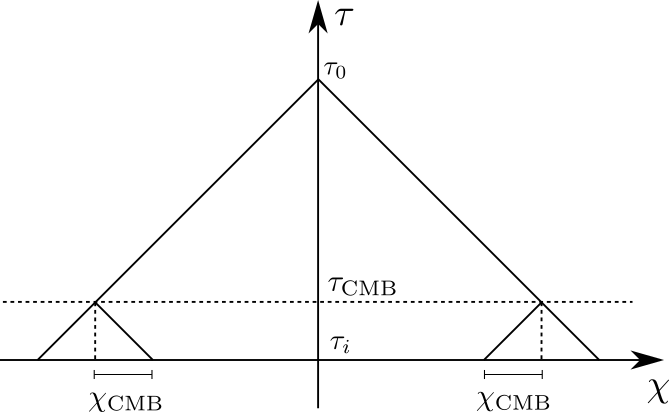
\includegraphics[width=0.7\textwidth]{horizon_problem.png}
	\caption{The horizon problem. According to the conventional big bang cosmology, different regions of the CMB we observe today have had no overlap in their particle horizon. Yet, the CMB is measured close to uniform everywhere.}
	\label{fig:horizon_problem}
\end{figure}

To resolve this issue, we need the particle horizon at recombination to be larger. The theory of cosmic inflation achieves this by having a period in the early universe where $3w+1<0$. In this case, we see from (\ref{eqn:particle_horizon_form}) that $\chi_\text{PH}$ is unbounded as $a_i \rightarrow 0$. The initial conformal time $\tau_i \rightarrow -\inf$, allowing enough proper time for the particle horizon growth. Then even the two opposite regions of the CMB we see can have had causal contact in the past, as depicted in Figure \ref{fig:horizon_solution}.
\begin{figure}[htbp!] 
	\centering    
	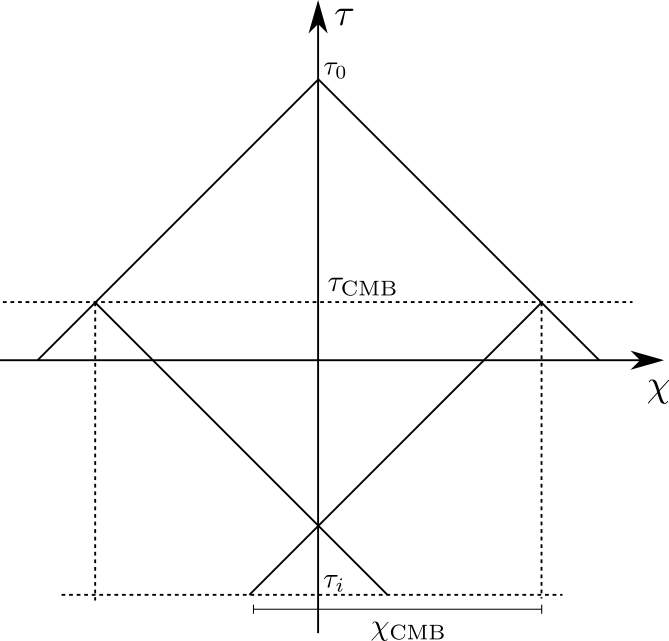
\includegraphics[width=0.6\textwidth]{horizon_solution.png}
	\caption{Solution to the horizon problem. Inflation allows more conformal time for different regions to have been in causal contact before recombination.}
	\label{fig:horizon_solution}
\end{figure}

Inflation can alternatively be characterised using the comoving Hubble radius defined as
\begin{align}
	\mathcal{H}^{-1} := \frac{1}{aH}.
\end{align}
Note that the particle horizon can then be expressed in terms of the comoving hubble radius as
\begin{align}
	\chi_\text{PH} = \int_{a_i}^{a_f} \frac{1}{a \dot{a}} da = \int_{\ln a_i}^{\ln a_f} \mathcal{H}^{-1} d\ln a. \label{eqn:particle_horizon_comoving_hubble}
\end{align}

The particle horizon represents the distance where objects could have \textit{ever} talked to each other. On the other hand, the comoving hubble radius is a scale for how far information can reach \textit{now}. \footnote{Two points $\mathcal{H}^{-1}$ apart drifts away with relative physical velocity $v_\text{phys} = \dot{a} \mathcal{H}^{-1} = 1$, which is equal to $c$ in our units. It is difficult for such points to have causal interaction right now, especially within Hubble time $H^{-1}$.} As can be seen from (\ref{eqn:particle_horizon_form}), $\mathcal{H}^{-1} \propto a^{(3w_X+1)/2}$, which is $\propto a$ for radiation domination and $\propto a^{1/2}$ during matter domination.

Inflation explains homogeneity of the observed CMB by requiring $\mathcal{H}^{-1}$ to have shrunk rapidly in early times; $d\mathcal{H}^{-1}/d\ln a < 0$. We find that $\ddot{a} > 0$, so the universe undergoes accelerated expansion. Steep decrease in $\mathcal{H}^{-1}$ is expressed using a `slow-roll' parameter
\begin{align}
	\epsilon := - \frac{d\ln H}{d\ln a} = -\frac{\dot{H}}{H^2} \ll 1. \label{def:slow_roll_epsilon}
\end{align}
Inflation also needs to last long enough for the particle horizon to grow sufficiently large. We define another parameter to denote this constraint;
\begin{align}
	\eta := \frac{d\ln \epsilon}{d\ln a} = \frac{\dot{\epsilon}}{\epsilon H} \ll 1. \label{def:slow_roll_eta}
\end{align}


\subsection{Slow-roll inflation}
\label{section:slow-roll_inflation}

The simplest model of inflation consists of a single scalar field $\phi$. The action for a real scalar field with canonical kinetic term and potential $V(\phi)$ is given by
\begin{align}
	S_\phi = \int dt d^3 \vv{x} \; \sqrt{-g} \left[ -\frac{1}{2} g^{\mu\nu} \partial_\mu \phi \partial_\nu \phi - V(\phi) \right],		\label{eqn:real_scalar_field_action}
\end{align}
where $g:=\det g$. Denoting the integrand as the Lagrangian density $\Lagr[t, \vv{x}, \phi, \partial_\mu \phi]$, the energy-momentum tensor can be expressed using functional derivatives as
\begin{align}
	T_{\mu\nu} = \frac{-2}{\sqrt{-g}} \frac{\delta\Lagr}{\delta g^{\mu\nu}} = -2 \frac{\delta \Lagr}{\delta g^{\mu\nu}} + g_{\mu\nu} \Lagr.
\end{align}
Here, we used the identity $\delta\sqrt{-g} = -(1/2) \sqrt{-g} g_{\mu\nu} \delta g^{\mu\nu}$. Substituting (\ref{eqn:real_scalar_field_action}),
\begin{align}
	T_{\mu\nu} = \left( \partial_\mu \phi \right) \left( \partial_\nu \phi \right) + g_{\mu\nu} \left( -\frac{1}{2} g^{\rho\sigma} \partial_\rho \phi \partial_\sigma \phi - V(\phi) \right).
\end{align}
Now suppose that $\phi$ drives inflation in the FLRW background. Due to the symmetries present in homogeneous and isotropic metric, the inflation field can only depend on time; $\phi(\vv{x}, t) = \bar{\phi}(t)$. We can read off the inflation field's energy density and pressure from the energy-momentum tensor.
\begin{align}
	\rho_{\bar{\phi}} =& -T^0_{\;\;0} = \frac{1}{2} \dot{\bar{\phi}}^2 + V(\bar{\phi}),	\\
	P_{\bar{\phi}} \delta^i_j =& T^i_{\;\;j} = \delta^i_j \left( \frac{1}{2} \dot{\bar{\phi}}^2 - V(\bar{\phi}) \right).
\end{align}
The two terms $\frac{1}{2} \dot{\bar{\phi}}^2$ and $V(\bar{\phi})$ can be interpreted as the kinetic and potential energy of inflation field, respectively. The equation of state is also expressed in terms of the two;
\begin{align}
	w_{\bar{\phi}} = \frac{P_{\bar{\phi}}}{\rho_{\bar{\phi}}} = \frac{\frac{1}{2} \dot{\bar{\phi}}^2 + V(\bar{\phi})}{\frac{1}{2} \dot{\bar{\phi}}^2 - V(\bar{\phi})}.
\end{align}
It follows that $\bar{\phi}$ satisfies the condition $3w_{\bar{\phi}}+1<0$ required for inflation, as long as the potential energy dominates over kinetic energy.

The classical equations of motion follows from the Euler-Lagrange equation. After some calculations we obtain
\begin{align}
	\ddot{\bar{\phi}} + 3H\dot{\bar{\phi}} = - V'(\bar{\phi}). 	  \label{eqn:inflation_background_equation_of_motion}
\end{align}
Even though $\bar{\phi}$ is a field, its dynamics given in (\ref{eqn:inflation_background_equation_of_motion}) are identical to those of a particle rolling down a one-dimensional potential. Its movement should be slow for the kinetic energy to be much smaller than the potential, and hence the name `slow-roll' inflation.

The Friedmann equations (\ref{eqn:Friedmann_1}-\ref{eqn:Friedmann_2}) can now be expressed in terms of the background inflationary field.
\begin{align}
	H^2 =& \frac{8\pi G}{3} \left( \frac{1}{2} \dot{\bar{\phi}}^2 + V(\bar{\phi}) \right) \approx \frac{8\pi G}{3} V(\bar{\phi}), \label{eqn:inflation_Friedmann_1} \\
	\frac{\ddot{a}}{a} =& -\frac{8\pi G}{3} \left( \dot{\bar{\phi}}^2 - \frac{1}{2} V(\bar{\phi}) \right) \approx \frac{8\pi G}{3} V(\bar{\phi}), \label{eqn:inflation_Friedmann_2}
\end{align}
where the slow-roll approximations have been used in the last step. Taking the derivative of (\ref{eqn:inflation_Friedmann_1}) gives us $3H\dot{\bar{\phi}} \approx -V'$. The parameters defined as
\begin{align}
	\epsilon_V := \frac{1}{16\pi G} \left( \frac{V'}{V} \right)^2, \;\;\;
	\eta_V := \frac{1}{8\pi G} \frac{V''}{V},
\end{align}
can then shown to be small. Therefore the slow roll parameters from (\ref{def:slow_roll_epsilon}-\ref{def:slow_roll_eta}) satisfy
\begin{align}
	\epsilon \approx \epsilon_V \ll 1, \;\;\;\;\; \eta \approx -2\eta_V + 4\epsilon_V \ll 1.
\end{align}
We see that as long as the potential $V(\phi)$ is chosen such that $\epsilon_V, \eta_V \ll 1$, the field $\phi$ can drive a period of accelerated expansion. Here, $\bar{\phi}(t)$ acts as a clock; it measures the progress of inflation, until $\epsilon$ eventually grows comparable to 1 and inflation ends.

\subsection{Quantum fluctuations} \label{section:quantum_fluctuations}

So far our considerations on the inflation field $\phi$ has been entirely classical. Moving on to quantum theory, field values are no longer fixed at each point in spacetime. The goal of this section is to quantify statistical properties of these quantum fluctuations.

We assume that the metric remains unperturbed for simplicity. Gravity is coupled with perturbations of the inflation field in reality, but this approximation will still allow us to derive most of the crucial results. We further neglect any terms suppressed by slow-roll parameters.

We write the inflation field as a sum of the classical solution and perturbation;
\begin{align}
	\phi(\vv{x}, t) = \bar{\phi}(t) + \frac{v(\vv{x}, t)}{a(t)},	\label{eqn:inflation_perturbation_definition}
\end{align}
where the factor of $1/a$ has been introduced for later convenience. First rewriting the scalar field action (\ref{eqn:real_scalar_field_action}) in terms of conformal time,
\begin{align}
	S_\phi = \int d\tau d^3\vv{x} a(\tau)^2 \left[ \frac{1}{2} (\phi')^2 - \frac{1}{2}(\nabla\phi)^2 - a(\tau)^2 V(\phi) \right].
\end{align}
When we include perturbations, terms linear in $v$ vanish from the equations of motion of $\bar\phi$. Further removing terms with derivatives of $V(\phi)$ using slow-roll condition,
\begin{align}
	\delta S_\phi =& \int d\tau d^3\vv{x} \left[ \frac{1}{2} \left(v' - \frac{a'}{a}v \right)^2 - \frac{1}{2}(\nabla v)^2 \right]	\\
	=& \int d\tau d^3\vv{x} \left[ \frac{1}{2} (v')^2 + \frac{1}{2}\frac{a''}{a} v^2 - \frac{1}{2}(\nabla v)^2 \right].
\end{align}
Integration by parts has been used to obtain the last line. The equations of motion for $v$ follows;
\begin{align}
	v'' - \frac{a''}{a} v - \nabla^2 v = 0.
\end{align}
Defining Fourier transforms of $v$ as
\begin{align}
	v(\vv{x},\tau) = \int \frac{d^3 \vv{k}}{(2\pi)^3} e^{i\vv{k} \cdot \vv{x}} \tilde{v}(\vv{k},\tau),
\end{align}
we obtain the Mukhanov-Sasaki equation;
\begin{align}
	v'' + (k^2 - \frac{a''}{a})v = 0	\label{eqn:Mukhanov_Sasaki}
\end{align}
Tildes above $v$ have been omitted for brevity. Each $\vv{k}$ mode of the perturbative field $v(\vv{k},\tau)$ evolves independently from each other. During slow-roll inflation $a\propto-1/\tau$, and $a''/a = 2/\tau^2$. General form of the solution is given by the \textit{mode functions} $v_k(\tau)$.
\begin{align}
	v_k(\tau) = c_+ \left( 1 - \frac{i}{k\tau} \right) e^{-ik\tau} + c_- \left( 1 + \frac{i}{k\tau} \right) e^{ik\tau}.
\end{align}

We would like to canonically quantise the field $v(\vv{k},\tau)$. To achieve this goal, we first convert from the Lagrangian to Hamiltonian formalism.
\begin{align}
	\pi :=& \frac{\partial \Lagr}{\partial v'} = v', \\
	\Hami :=& v'\frac{\partial \Lagr}{\partial v'} - \Lagr = \frac{1}{2} \pi^2 + \frac{1}{2} (\nabla v)^2 - \frac{1}{2} \frac{a''}{a} v^2 .
\end{align}
We now promote classical fields $v(\vv{k},\tau)$, $\pi(\vv{k},\tau)$ to operators $\hat{v}_\vv{k}(\tau)$, $\hat{\pi}_\vv{k}(\tau)$ satisfying equal-time commutation relations \footnote{This follows from its Fourier equivalent: $[\hat{v}(\vv{x}_1,\tau),\hat{\pi}(\vv{x}_2,\tau)] = i\delta^{(3)}(\vv{x}_1 - \vv{x}_2)$.}
\begin{align}
	\left[ \hat{v}_{\vv{k}_1}(\tau), \hat{\pi}_{\vv{k}_2}(\tau) \right] =& (2\pi)^3 \delta^{(3)}(\vv{k}_1 + \vv{k}_2), \\
	\left[ \hat{v}_{\vv{k}_1}(\tau), \hat{v}_{\vv{k}_2}(\tau) \right] =& \left[ \hat{\pi}_{\vv{k}_1}(\tau), \hat{\pi}_{\vv{k}_2}(\tau) \right] = 0.
\end{align}
Defining operators $\hat{a}_\vv{k}$ and $\hat{a}_\vv{k}^\dagger$ appropriately, we may write
\begin{align}
	\hat{v}_\vv{k} (\tau) =& v_k(\tau) \hat{a}_\vv{k} + v_k(\tau)^* \hat{a}_{-\vv{k}}^\dagger,  \\
	\hat{\pi}_\vv{k} (\tau) =& {v'_k}(\tau) \hat{a}_\vv{k} + {v'_k}(\tau)^* \hat{a}_{-\vv{k}}^\dagger.
\end{align}
As long as we normalise the mode functions $v_k(\tau)$ so that its Wronskian $W := v_k v'^*_k - v_k^* v'_k = i$ (purely imaginary since $v_k$ is real), we obtain
\begin{align}
	\left[ \hat{v}_{\vv{k}_1}(\tau), \hat{\pi}_{\vv{k}_2}(\tau) \right] =& i \left[ \hat{a}_{\vv{k}_1}, \hat{a}^\dagger_{\vv{k}_2} \right], \\
	\left[ \hat{a}_{\vv{k}_1}, \hat{a}^\dagger_{\vv{k}_2} \right] =& (2\pi)^3 \delta^{(3)}(\vv{k}_1 - \vv{k}_2).	\label{eqn:canonical_quantisation_commutation_relation_a}
\end{align}
The constructed $\hat{a}$ and $\hat{a}^\dagger$ are analogous to the creation and annihilation operators of quantum harmonic oscillator. Our next step is to compute the Hamiltonian operator;
\begin{align}
	\hat{H} =& \int d^3 \vv{x} \left[ \frac{1}{2} \hat{\pi}^2 + \frac{1}{2} \left( \nabla \hat{v} \right)^2 - \frac{1}{2}\frac{a''}{a} \hat{v}^2 \right] \label{eqn:single_field_inflation_simple_hammiltonian}\\
	=& \int d^3 \vv{x} \frac{d^3 \vv{k}_1}{(2\pi)^3} \frac{d^3 \vv{k}_2}{(2\pi)^3} \frac{1}{2} e^{i(\vv{k}_1 + \vv{k}_2) \cdot \vv{x}}  \left[ \hat{\pi}_{\vv{k}_1} \hat{\pi}_{\vv{k}_2} - (\vv{k_1} \cdot \vv{k_2}) \hat{v}_{\vv{k}_1} \hat{v}_{\vv{k}_2} - \frac{a''}{a} \hat{v}_{\vv{k}_1} \hat{v}_{\vv{k}_2} \right] \\
	=& \int \frac{d^3 \vv{k}}{(2\pi)^3}  \frac{1}{2} \left[ \hat{\pi}_{\vv{k}} \hat{\pi}_{-\vv{k}} + k^2 \hat{v}_{\vv{k}} \hat{v}_{-\vv{k}} - \frac{a''}{a} \hat{v}_{\vv{k}} \hat{v}_{-\vv{k}} \right] \\
	=&  \int \frac{d^3 \vv{k}}{(2\pi)^3} \left[ E_k \left( \hat{a}_\vv{k} \hat{a}^\dagger_\vv{k} + \hat{a}^\dagger_{-\vv{k}} \hat{a}_{-\vv{k}} \right) + F_k \hat{a}_{\vv{k}} \hat{a}_{-\vv{k}} + F_k^* \hat{a}^\dagger_{\vv{k}} \hat{a}^\dagger_{-\vv{k}}  \right],
\end{align}
where
\begin{align}
	\omega_k^2 := k^2 - \frac{a''}{a}, \;\;\; E_k := \frac{1}{2}(|v'_k|^2 + \omega_k^2 |v_k|^2), \;\;\; F_k := \frac{1}{2}(v'^2_k + \omega_k^2 v^2_k).
\end{align}

Note that we are currently in Heisenberg picture where the operators depend on time. Our mode functions have two degrees of freedom: $c_+$ and $c_-$. One of them has been fixed by the normalisation condition $W=2ik(|c_+|^2-|c_-|^2)=i$. The other degree of freedom remains, availing us one-parameter family of possible initial mode functions. Note that $\hat{a}^\dagger_\vv{k}$ are defined in terms of $\hat{v}_\vv{k}$ and $\hat{\pi}_\vv{k}$. Fixing $\hat{a}_\vv{k}$ is thus equivalent to choosing $\hat{v}_\vv{k}$.

We define the vacuum $|\vv{0}\rangle$ to be the state satisfying $\hat{a}_\vv{k} |\vv{0}\rangle = 0$ for all $\vv{k} \in \mathbb{R}^3$. The expected energy of the vacuum state is given by
\begin{align}
	\langle \vv{0} | \hat{H} | \vv{0} \rangle =& \int \frac{d^3\vv{k}}{(2\pi)^3} E_k \langle \vv{0} | [ \hat{a}_\vv{k}, \hat{a}^\dagger_\vv{k} ] | \vv{0} \rangle	\\
	=& \int d^3\vv{k} E_k \delta^{(3)}(0),
\end{align}
where the divergence $\delta^{(3)}(0)$ arises only because we are integrating over the whole space. Removing this factor, we may interpret $E_k$ as the vacuum energy density for mode $k$.

We now ask the vacuum state to be a ground state of the Hamiltonian. Minimising the energy density $E_k$ while keeping normalisation condition $W=i$, we obtain the \textit{Bunch-Davies} mode function;
\begin{align}
	v_\vv{k}(\tau) = \frac{1}{\sqrt{2k}} \left( 1 - \frac{i}{k\tau} \right) e^{-ik\tau}. \label{eqn:bunch_davis_mode_function}
\end{align}
For this choice of mode function and vacuum, $E_k \rightarrow \hslash\omega_k/2$ as $\tau \rightarrow -\infty$. \footnote{$\hslash$ has been reinstated here for clarity.} This is analogous to the case of quantum harmonic oscillator.

Lastly, we compute zero-point fluctuation of the inflation field with respect to the vacuum. The two-point function follows from the commutation relation \eqref{eqn:canonical_quantisation_commutation_relation_a};
\begin{align}
	\langle \hat{v}_{\vv{k}_1} (\tau) \hat{v}_{\vv{k}_2} (\tau) \rangle &= \langle 0| [\hat{a}_{\vv{k}_1}, \hat{a}^\dagger_{-\vv{k}_2}] |0 \rangle \; v_{k_1}(\tau) v^*_{k_2}(\tau) \\
	&= (2\pi)^3 \delta^{(3)} (\vv{k}_1 + \vv{k}_2 ) \; P_{v}(k_1,\tau),   \label{eqn:single_field_inflation_power_spectrum}
\end{align}
where we defined the \textit{power spectrum} of $v$ as $P_v(k,\tau) := |v_k(\tau)|^2$. Fourier transforming back using
\begin{align}
	\hat{v}(\vv{x}, \tau) = \int \frac{d^3\vv{k}}{(2\pi)^3} \left[ v_k \hat{a}_\vv{k} + v^*_k \hat{a}^\dagger_\vv{k} \right] e^{i\vv{k} \cdot \vv{x}},
\end{align}
we compute the local variation in $v$;
\begin{align}
	\langle | \hat{v}(\vv{x}, \tau) |^2 \rangle =& \int \frac{d^3\vv{k}_1}{(2\pi)^3} \frac{d^3\vv{k}_2}{(2\pi)^3} \langle \vv{0} | v_{k_1} \hat{a}_{\vv{k}_1} v^*_{k_2} \hat{a}^\dagger_{\vv{k}_2} | \vv{0} \rangle 	\\
	=& \int \frac{d^3\vv{k}_1}{(2\pi)^3} \frac{d^3\vv{k}_2}{(2\pi)^3} v_{k_1} v^*_{k_2} \langle \vv{0} | \left[ \hat{a}_{\vv{k}_1}, \hat{a}^\dagger_{\vv{k}_2} \right] | \vv{0} \rangle	 \\
	=& \int \frac{d^3\vv{k}}{(2\pi)^3} |v_k|^2	\\
	=& \int d(\ln k) \mathcal{P}_v (k,\tau).
\end{align}
The dimensionless power spectrum is defined as
\begin{align}
	\mathcal{P}_v (k,\tau) := \frac{k^3}{2\pi^2} P_v(k,\tau).
\end{align}
Recall that perturbations in $\phi$ is given by $\delta\phi = v/a$ from (\ref{eqn:inflation_perturbation_definition}). The \textit{dimensionless power spectrum} for fluctuations in $\phi$ is therefore
\begin{align}
	\mathcal{P}_{\delta\phi} (k,\tau) = \frac{\mathcal{P}_v (k,\tau)}{a(\tau)^2} = \left( \frac{H}{2\pi} \right)^2 \left(1 + (k\tau)^2 \right),
\end{align}
where we used the fact that $a(\tau) = -1/H\tau$ during slow-roll inflation. For scales larger than the comoving Hubble radius we have $k\tau \ll 1$. In this limit, $\mathcal{P}_{\delta\phi} \rightarrow (H/2\pi)^2$ which is nearly constant. This is a key prediction from our simplistic model of inflation; we expect a near scale-invariant power spectrum of the primordial (end-of-inflation) perturbations.



\section*{Summary}

In this introductory chapter we covered the basic foundations of modern cosmology. Under a simplifying assumption that the universe is homogeneous and isotropic, we wrote down the most general metric tensor in which the scale factor $a(t)$ parametrises the expansion of the universe. We then considered radiation, matter and dark energy as main constituents of the universe and derived Friedmann equations, which can be solved to determine the universe's expansion history given its energy composition. In particular, the universe likely began with a Big Bang and has been continuously expanding since. This led to another puzzle, the horizon problem; the early universe observed through CMB seems exceptionally uniform despite supposedly having many casually disconnected regions. We discussed how inflation solves the problem by introducing a period of accelerated expansion shortly after Big Bang, dramatically increasing the size of particle horizon. Inflation also successfully provides a mechanism for generating initial fluctuations in the universe. We showed that quantum fluctuations in the inflation field follow a near scale-invariant spectrum which is consistent with observations to date.

The universe observed today is not quite homogeneous and isotropic at all scales. In fact, it is the inhomogeneities\textemdash perturbations about the homogeneous background\textemdash that contain valuable information of the universe and are crucial observables for precision cosmology. We formulate the cosmological perturbation theory in the following chapter in the context of the CMB.